\section{Pianificazione}
Lo sviluppo del progetto è costruito sulla base delle scadenze riportate nella sottosezione \textsection1.5 ed è suddiviso nelle seguenti fasi:
\begin{itemize}
	\item analisi;
	\item consolidamento dei requisiti
	\item progettazione architetturale;
	\item progettazione di dettaglio e codifica;
	\item validazione e collaudo.
\end{itemize}

\subsection{Analisi}
\textbf{Periodo}: dal 2020-03-10 al 2020-04-13 \\
Questo periodo ha inizio con la formazione dei gruppi e termina con la scadenza per la consegna dei documenti relativi alla \textit{Revisione dei Requisiti}. \\
Le principali attività svolte in questo periodo sono:
\begin{itemize}
	\item \textbf{Strumenti di lavoro}: questa attività consiste nella scelta degli strumenti di lavoro da utilizzare per lo svolgimento del progetto;
	\item \textbf{\NdP{}}: attività nella quale gli Amministratori redigono le \textit{\NdP{}}, documento in cui si specificano tutte le regole, le convenzioni e le tecnologie che i componenti del gruppo adotteranno durante tutto il corso del progetto. Questa attività include una stesura iniziale del documento, comprensiva delle norme e degli standard accordati dal gruppo, il documento verrà poi ampliato in base all'individuazione di sezioni da ampliare;
	\item \textbf{\SdF{}}: attività nella quale gli Analisti redigono lo \textit{\SdF}, documento in cui vengono analizzati i capitolati d'appalto elencando per ciascuno i punti positivi e negativi che li caratterizzano. Inoltre vengono indicate le motivazioni per le quali è stato scelto il capitolato\ped{\textit{G}} C2 denominato \textit{Etherless} e sono stati esclusi i capitolati restanti. \\
	Questa attività è bloccante per l'inizio dell'\textit{\AdR{}};
	\item \textbf{\AdR{}}: attività nella quale gli Analisti redigono l'\textit{\AdR{}}, documento essenziale in cui viene analizzato in maniera approfondita il capitolato\ped{\textit{G}} scelto a seguito dello \textit{\SdF}, individuando le funzionalità e i casi d'uso previsti dal progetto;
	\item \textbf{\PdP{}}: attività nella quale il Responsabile redige il \textit{\PdP}, documento in cui viene presentata la pianificazione del gruppo per lo sviluppo del progetto, un'analisi dei rischi e dei costi e dove vengono indicate le scadenze che il gruppo intende rispettare per la buona riuscita del progetto;
	\item \textbf{\PdQ{}}: attività nella quale gli Analisti redigono il \textit{\PdQ}, documento in cui vengono indicate tutte le strategie di verifica e validazione che il gruppo intende adottare con lo scopo di garantire la qualità di processo e di prodotto\ped{\textit{G}};
	\item \textbf{\Glossario{}}: attività nella quale viene redatto il \textit{\Glossario}, documento nel quale verranno elencati, chiariti ed approfonditi tutti i termini tecnici utilizzati nei documenti con lo scopo di evitare possibili ambiguità;
	\item \textbf{Lettera di Presentazione}: attività nella quale viene redatta la \textit{Lettera di Presentazione} necessaria per la presentazione come fornitore del gruppo.
\end{itemize}
	\subsubsection{Diagramma di Gantt: Analisi}
		\begin{figure}[h]
			\centering
			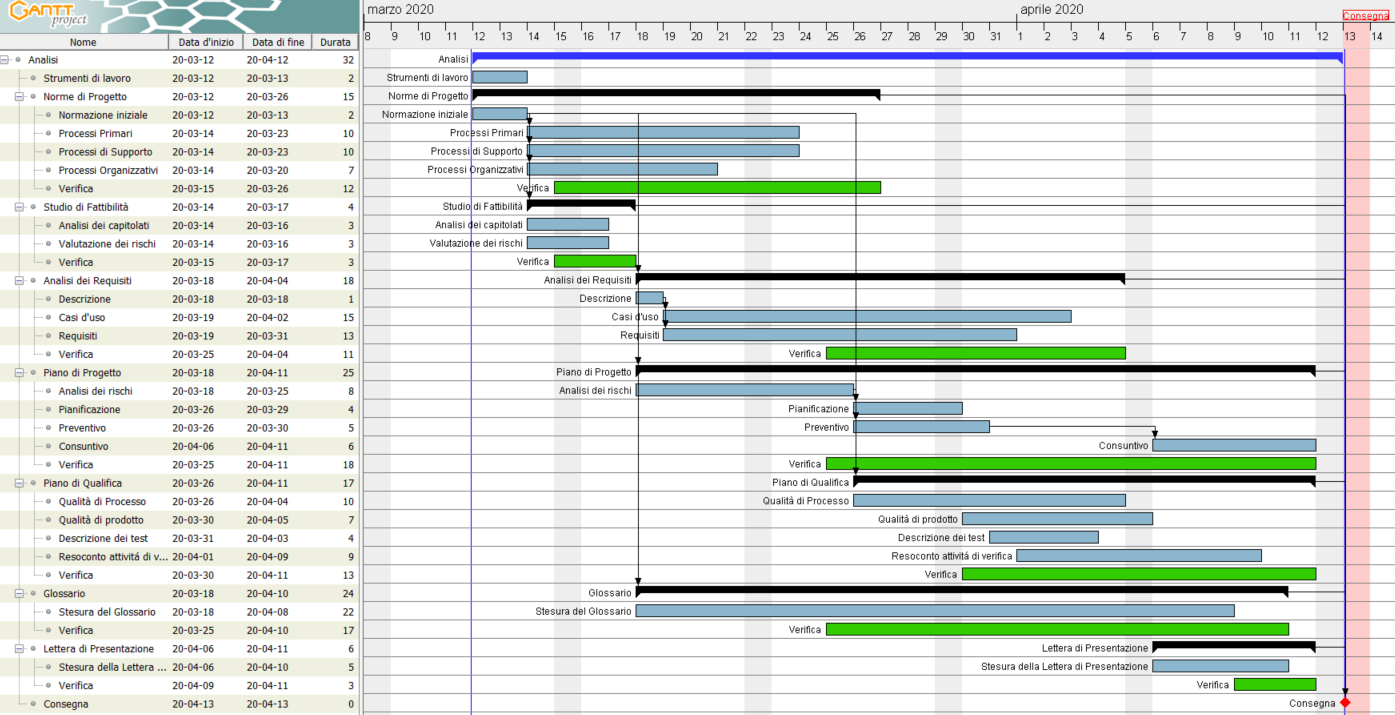
\includegraphics[width=1.1\textwidth]{./res/img/DiagrammiGantt/analisi_gantt.png}
			\caption{Diagramma di Gantt del periodo di Analisi}
		\end{figure}

\subsection{Consolidamento dei Requisiti}
\textbf{Periodo}: dal 2020-04-13 al 2020-04-20 \\
Questo periodo ha inizio dopo il termine del periodo di Analisi e termina il giorno della presentazione della \textit{Revisione dei Requisiti}. \\
%In questo periodo l'attivita principale prevede un consolidamento e un miglioramento dei requisiti ottenuti conclusa la fase di analisi e una preparazione del materiale necessario alla presentazione del 2020-04-20. \\
%Inoltre, qualora se ne presentasse la necessità verranno apportate modifiche migliorative ai documenti redatti durante la fase precedente.
\begin{itemize}
	\item \textbf{Incremento e Verifica dei documenti:} in caso di necessità, vengono migliorati e verificati i documenti preparati nella fase precedente;
	\item \textbf{Consolidamento Analisi dei requisiti}: l'attività principale, prevede un consolidamento e un miglioramento dei requisiti ottenuti conclusa la fase di Analisi e conseguente aggiornamento dell'\textit{\AdR{}};
	\item \textbf{Realizzazione della presentazione:} preparazione del materiale necessario alla presentazione del 2020-04-20.
\end{itemize}
	\subsubsection{Diagramma di Gantt: Consolidamento dei Requisiti}
		\begin{figure}[h]
			\centering
			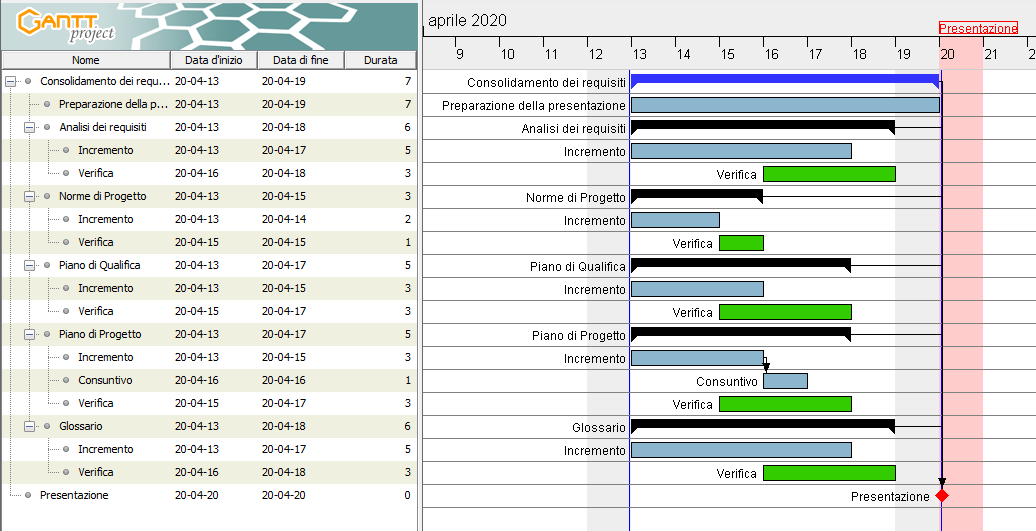
\includegraphics[width=1.1\textwidth]{./res/img/DiagrammiGantt/cons_req_gantt.png}
			\caption{Diagramma di Gantt del periodo di Consolidamento dei Requisiti}
		\end{figure}
\newpage
\subsection{Progettazione Architetturale}
\textbf{Periodo}: dal 2020-04-20 al 2020-05-11 \\
Questo periodo ha inizio al termine del periodo di Consolidamento dei Requisiti e termina con la scadenza per la consegna dei documenti relativi alla \textit{Revisione di Progettazione}. \\
Questo periodo porta all'individuazione di una soluzione architetturale che permetta il soddisfacimento dei requisiti individuati.
\begin{itemize}
	\item \textbf{Incremento e verifica}: come prima cosa, analizzando l'esito della \textit{Revisione dei Requisiti} vengono svolte attività di incremento e verifica sui vari documenti redatti, dove necessario. \\
	L'incremento dell'\textit{\AdR{}} è il più importante perchè va completato prima di poter proseguire con il resto delle attività;
	\item \textbf{Technology Baseline}: viene redatta la documentazione di supporto, contenente la descrizione delle tecnologie individuate e il tracciamento della relazione tra le componenti e i requisiti che vanno a soddisfare. Viene anche codificato il \textbf{PoC (Proof of Concept)} come dimostrazione del funzionamento dell'architettura individuata;
	\item \textbf{Glossario}: attività che prevede un miglioramento del \textit{Glossario} aggiungendo nuovi termini oppure raffinando le definizioni di termini già presenti.
\end{itemize}
	\subsubsection{Diagramma di Gantt: Progettazione Architetturale}
		\begin{figure}[h]
			\centering
			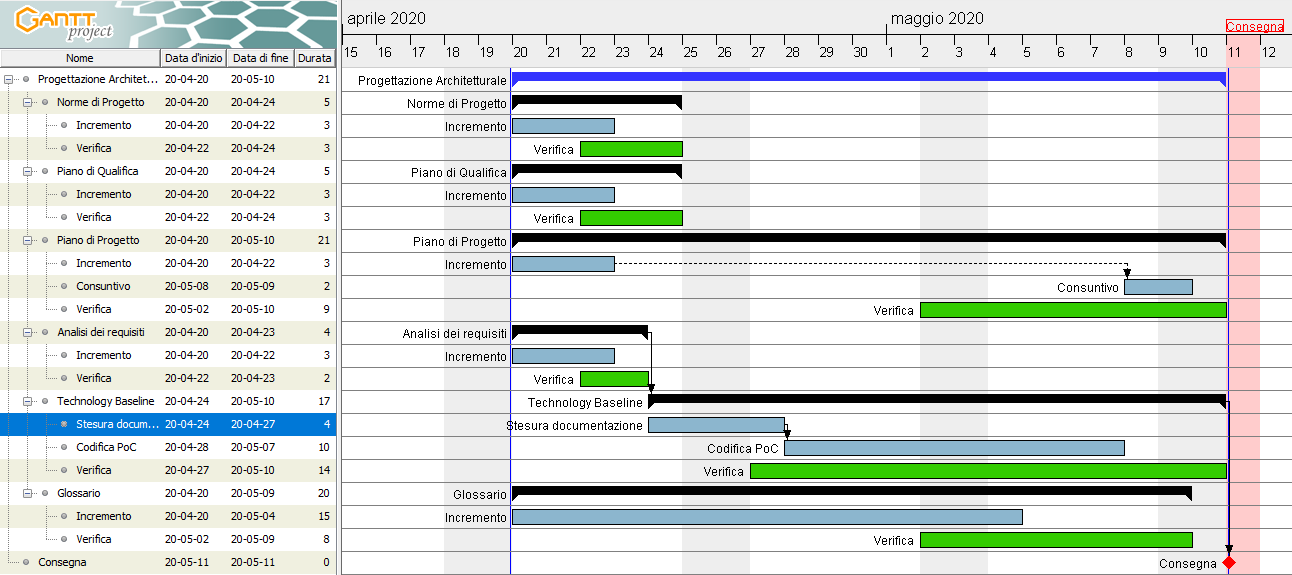
\includegraphics[width=1.1\textwidth]{./res/img/DiagrammiGantt/prog_arch_gantt.png}
			\caption{Diagramma di Gantt del periodo di Progettazione Architetturale}
		\end{figure}
\newpage
\subsection{Progettazione di Dettaglio e Codifica}
\textbf{Periodo}: dal 2020-05-11 al 2020-06-11 \\
Questo periodo ha inizio dopo il termine del periodo di Progettazione Architetturale, quindi alla scadenza della consegna della \textit{Revisione di Progettazione} e termina con la scadenza per la consegna dei documenti relativi alla \textit{Revisione di Qualifica}. \\
Le principali attività svolte in questo periodo sono:
\begin{itemize}
	\item \textbf{Incremento e verifica}: come prima cosa, analizzando l'esito della \textit{Revisione dei Progettazione} vengono svolte attività di incremento e verifica sui vari documenti redatti;
	\item \textbf{Product Baseline}: progettazione dettagliata a basso livello delle componenti del prodotto\ped{\textit{G}}, coerente con quanto individuato nella Technology Baseline;
	\begin{itemize}
		\item \textbf{Allegato Tecnico}: stesura del documento di \textit{Allegato Tecnico}, di supporto alla progettazione di dettaglio;
		\item \textbf{Codifica}: attività nella quale viene prodotto\ped{\textit{G}} e verificato il codice.
	\end{itemize}
	\item \textbf{User Manual}(manuale utente): attività nella quale viene redatto lo \textit{User Manual} contenente le informazioni su come funziona e su come si utilizza il prodotto\ped{\textit{G}};
	\item \textbf{Glossario}: attività che prevede un miglioramento del \textit{Glossario} aggiungendo nuovi termini oppure raffinando le definizioni di termini già presenti.
\end{itemize}
	\subsubsection{Diagramma di Gantt: Progettazione di Dettaglio e Codifica}
		\begin{figure}[h]
			\centering
			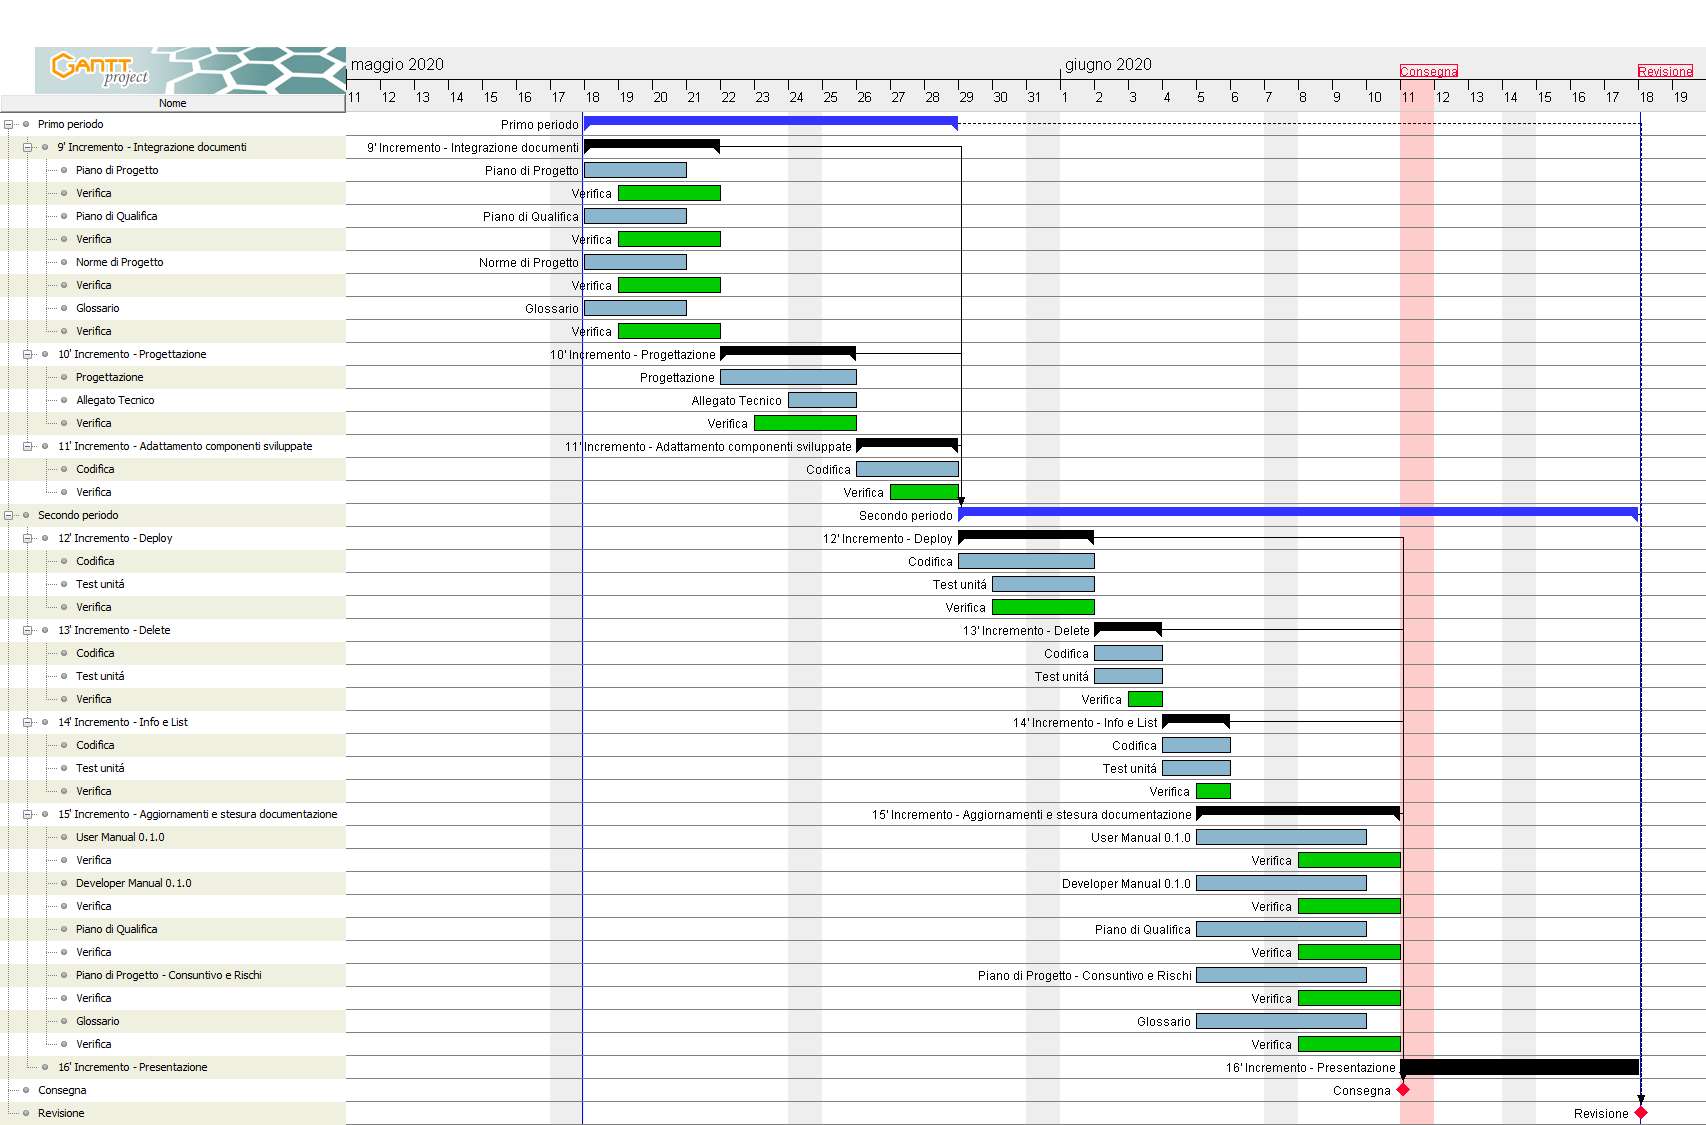
\includegraphics[width=1.1\textwidth]{./res/img/DiagrammiGantt/prog_dett_gantt.png}
			\caption{Diagramma di Gantt del periodo di Progettazione di Dettaglio e Codifica}
		\end{figure}
\newpage
\subsection{Validazione e Collaudo}
\textbf{Periodo}: dal 2020-06-11 al 2020-07-13 \\
Questo periodo ha inizio dopo il termine del periodo di Progettazione di Dettaglio e Codifica e termina con la scadenza per la consegna dei documenti relativi alla \textit{Revisione di Accettazione}. \\
Le principali attività svolte in questo periodo sono:
\begin{itemize}
	\item \textbf{Incremento e verifica}: come prima cosa, analizzando l'esito della \textit{Revisione dei Qualifica} vengono svolte attività di incremento e verifica sui vari documenti redatti;
	\item \textbf{Validazione e Collaudo}: attività nella quale vengono eseguiti test e, se necessario, vengono apportati dei miglioramenti al prodotto\ped{\textit{G}} per poter assicurare il soddisfacimento dei requisiti e dei vincoli qualitativi;
	\item \textbf{User Manual}: attività nella quale viene migliorato lo \textit{User Manual};
	\item \textbf{Manuale Sviluppatore}: attività nella quale viene redatto il \textit{Manuale Sviluppatore}, il quale contiene le informazioni utili al mantenimento del prodotto\ped{\textit{G}};
	\item \textbf{Glossario}: attività che prevede un miglioramento del \textit{Glossario} aggiungendo nuovi termini oppure raffinando le definizioni di termini già presenti.
\end{itemize}
	\subsubsection{Diagramma di Gantt: Validazione e Collaudo}
		\begin{figure}[h]
			\centering
			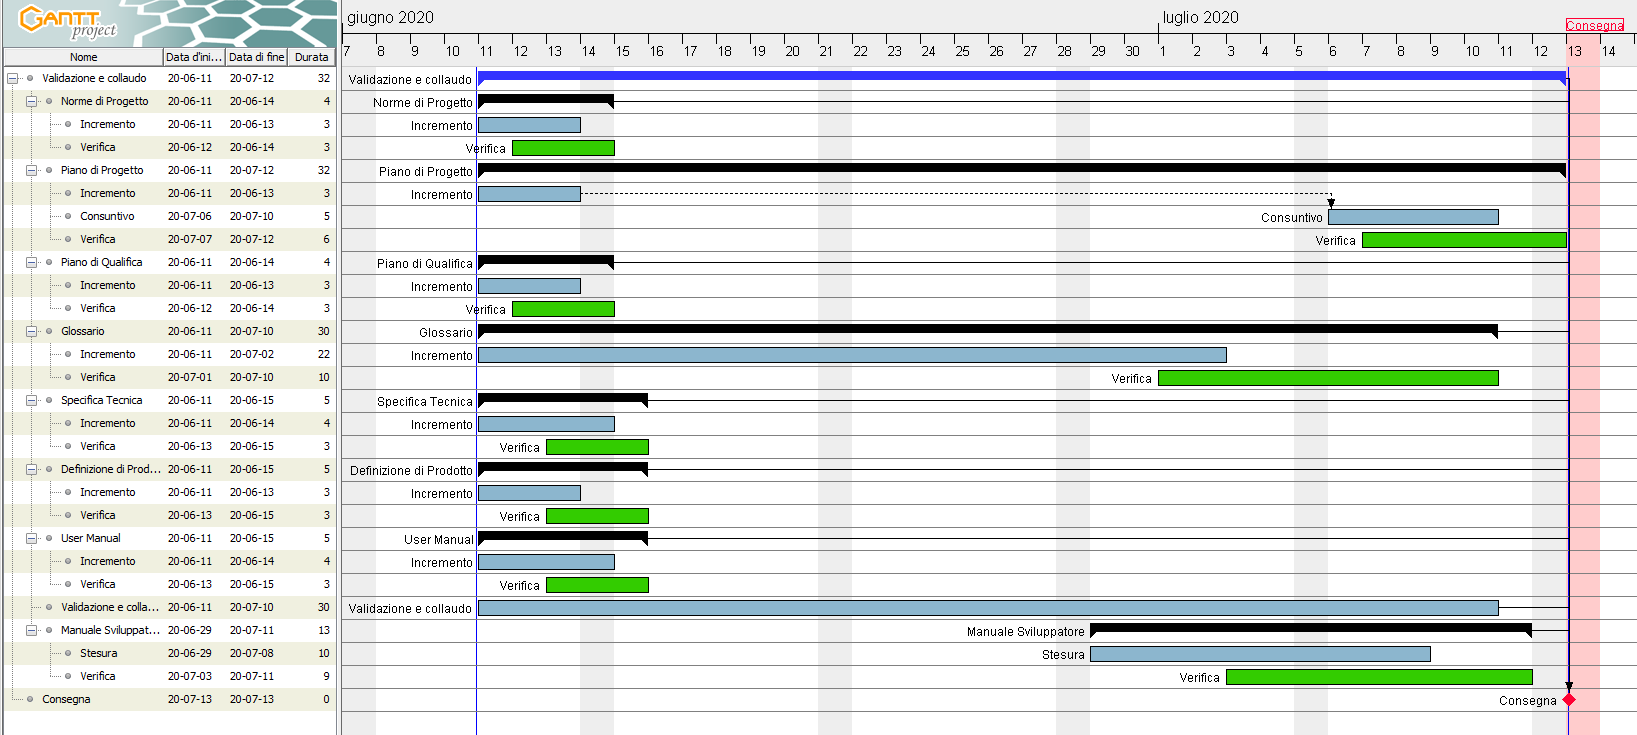
\includegraphics[width=1.1\textwidth]{./res/img/DiagrammiGantt/validaz_gantt.png}
			\caption{Diagramma di Gantt del periodo di Validazione e Collaudo}
		\end{figure}
